\section{Multi-Agent Source Localization}
\label{sec:04_multiAgentLoca}

After the three \ac{TDOA} methods \ac{CC}, \ac{GCC} and phase difference were
evaluated in the preceding sections, the \ac{SSL} algorithm with a multi-agent system
of five robots is evaluated.
The remaining part of this chapter focuses on the performance of the \ac{SSL}
with regard to each \ac{TDOA} method individually.
Input to the \ac{SSL} algorithm are the \ac{WSDE} of each
robot in the team. Based on these results, the multi-agent whistle localization outputs
an absolute sound source position in field coordinates.
To provide a decoupled result to the signal start detection,
the start indexes were set manually.
In the following, the laboratory-measurements of \Cref{subsec:04_labMeasurements}
are utilized for evaluation of all methods.

% -------------------------------------------------------------
\subsection{CC Method}
\label{04_teamCc}


To determine an overall result, each robot computes a direction prediction from
the locally recorded signal using the \ac{GCC-PHAT} method standing
alone.
These local direction estimates of individual robots are fed to the team
decision filter as specified in \cref{sec:03_multiAgentLoca} which estimates the
global sound source position by combining all measurements through Bayesian
updates.
First, the results of the \ac{SSL} algorithm are presented with
the \ac{WSDE} calculated by simple \ac{CC}.
The results for the predictions of this method are reported in
\Cref{tab:04_ccTeamResult} lists the error of the localized position
in regard to the real sound source position in x- and y-coordinates.
Additionally, the angular error in field coordinates is listed.
It indicates if the result has a correct tendency.

% -------------------------------------------------------------
\btline{ht}{1.2}
\btab{|c|c|c|c|c|c|}
\hline
& & Error & Error & Error & Error\\
No. & Measurement & x [\si{\meter}] & y [\si{\meter}] & Abs. Distance [\si{\meter}] & Angle\\
\hline
0 & front left & 0.6 & 1.39 & 1.51 & 8.15\si{\degree}\\
\hline
1 & front right & -0.49 & 1.2 & 1.3 & 11.97\si{\degree}\\
\hline
2 & rear right & 2.32 & 2.11 & 3.13 & 18.28\si{\degree}\\
\hline
3 & rear left & 1.07 & -0.96 & 1.44 & 3.71\si{\degree}\\
\hline
4 & own penalty spot & 1.95 & -0.09 & 1.95 & 10.44\si{\degree}\\
\hline
5 & opponent penalty spot & 0.07 & 0.01 & 0.07 & 0.32\si{\degree}\\
\hline
6 & center & 0.4 & -0.01 & 0.4 & 1.91\si{\degree}\\
\hline
7 & center right & 1.06 & -0.0 & 1.06 & 22.99\si{\degree}\\
\hline
8 & behind own goal & 1.24 & -0.06 & 1.24 & 0.77\si{\degree}\\
\hline
9 & rear left & -0.04 & 0.78 & 0.78 & 7.22\si{\degree}\\
\hline
10 & center & 0.03 & -0.0 & 0.03 & 0.0\si{\degree}\\
\hline
\etab
\et{Whistle localization results of laboratory-measurements with
\ac{CC} method}{04_ccTeamResult}
% -------------------------------------------------------------

Over all measurements, the \ac{CC} predictor has
a \ac{RMSE} of 1.45\si{\meter} in distance and 10.67\si{\degree} angular.

\subsection{GCC Method}
\label{04_teamGcc}

As the \ac{GCC} method provides the best results for the \ac{WSDE} results,
more precise steps of the multi-agent source localization algorithm are presented
here.
For further clarification, measurement 1 of the laboratory-measurements is
selected as example.
\Cref{fig:04_gccResult} illustrates the result of the relative direction
estimates $\gamma_i$ of the individual robots listed in \cref{tab:04_gccResult}
for this example.
For \cref{fig:04_setup,fig:04_gccResult}, robot positions are marked by yellow dots
where a short yellow line indicates each robot's orientation.
The arrows in \cref{fig:04_gccResult} represent the local direction estimates
$\gamma_i$ as predicted by each robot. Finally, the true position of the sound
source is marked with a red star while the joint position estimate over all
robots is visualized by a cross.
% -------------------------------------------------------------
\btline{ht}{1.2}
\btab{|c|c|c|c|}
\hline
NAO & $\gamma_i$ & Abs. Error\\
\hline
21 & -26.22\si{\degree} & 3.71\si{\degree}\\
\hline
24 & -133.77\si{\degree} & 9.32\si{\degree}\\
\hline
26 & -30.19\si{\degree} & 3.50\si{\degree}\\
\hline
27 & -75.26\si{\degree} & 1.71\si{\degree}\\
\hline
28 & -15.90\si{\degree} & 2.53\si{\degree}\\
\hline
\etab
\et{Resulting direction estimates of the individual robots with \ac{GCC-PHAT}
method for a whistle-sound signal in the right front corner of the playing
field}{04_gccResult}
% -------------------------------------------------------------
\begin{figure}[H]
	\centering
		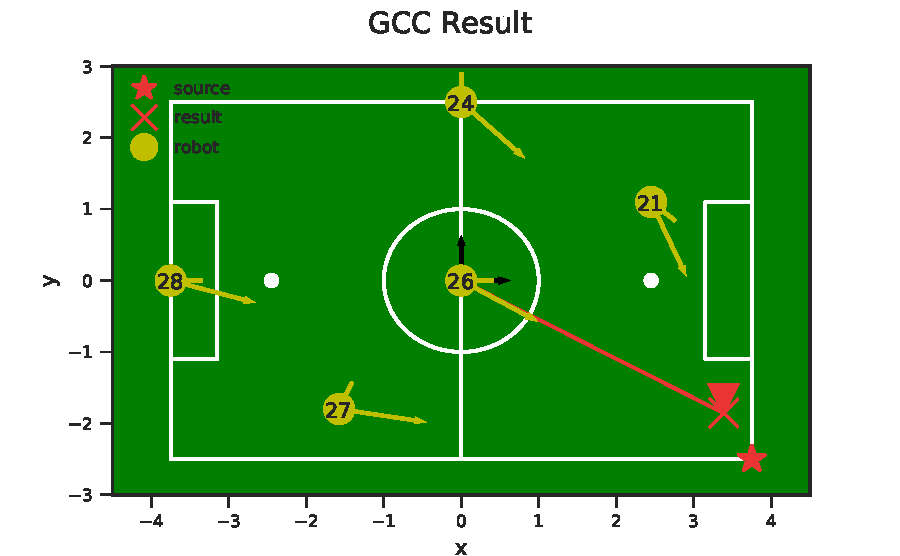
\includegraphics[]{figures/evaluation/gcc_team}
	\caption{Team whistle localization result with \ac{GCC-PHAT}
	method.}
    \label{fig:04_gccResult}
\end{figure}
% -------------------------------------------------------------

The final result and its corresponding errors are listed in
\cref{tab:04_gccTeamResult}.
% -------------------------------------------------------------
\btline{H}{1.2}
\btab{|c|c|c|}
\hline
 & Result & Error\\
\hline
Position x [\si{\meter}] & 3.38 & -0.37\\
\hline
Position y [\si{\meter}] & -1.85 & 0.65\\
\hline
Angle & 33.18\si{\degree} & 1.57\si{\degree}\\
\hline
Distance [\si{\meter}] & 3.85 & 0.74 \\
\hline
\etab
\et{Whistle localization result of measurement 1 with \ac{GCC-PHAT} method}{04_gccTeamResult}
% -------------------------------------------------------------

\Cref{tab:04_gccTeamResult} shows the distance and angle errors
for all laboratory measurements in \cref{subsec:04_labMeasurements}.
The \ac{RMSE} of the localized source positions in distance being 0.87\si{\meter}
and angular \ac{RMSE} being 5.07\si{\degree} one can say that the \ac{GCC-PHAT} algorithm
works well for whistle-sound source localization.
% -------------------------------------------------------------

\btline{ht}{1.2}
\btab{|c|c|c|c|c|c|}
\hline
& & Error & Error & Error & Error\\
No. & Measurement & x [\si{\meter}] & y [\si{\meter}] & Abs. Distance [\si{\meter}] & Angle\\
\hline
0 & front left & 1.31 & 1.06 & 1.68 & 1.45\si{\degree}\\
\hline
1 & front right & 0.13 & 0.06 & 0.15 & 1.57\si{\degree}\\
\hline
2 & rear right & 0.59 & 0.43 & 0.73 & 0.42\si{\degree}\\
\hline
3 & rear left & 0.54 & 0.47 & 0.72 & 9.09\si{\degree}\\
\hline
4 & own penalty spot & 0.27 & 0.0 & 0.27 & 0.01\si{\degree}\\
\hline
5 & opponent penalty spot & 0.15 & 0.14 & 0.21 & 3.18\si{\degree}\\
\hline
6 & center & 0.41 & -0.02 & 0.41 & 2.67\si{\degree}\\
\hline
7 & center right & 0.39 & 0.02 & 0.39 & 8.98\si{\degree}\\
\hline
8 & behind own goal & 1.84 & -0.01 & 1.84 & 0.14\si{\degree}\\
\hline
9 & rear left & 0.58 & 0.52 & 0.78 & 9.89\si{\degree}\\
\hline
10 & center & 0.03 & -0.0 & 0.03 & 0.0\si{\degree}\\
\hline
\etab
\et{Whistle localization results for all laboratory-measurements with
\ac{GCC-PHAT} method}{04_gccTeamResult}
% -------------------------------------------------------------
% - intersections
% - updates
% - covariance
% - PSNR

% -------------------------------------------------------------
\subsection{Phase Method}
\label{04_teamPhase}

Finally, the performance  of the phase method is evaluated.
In this experiment, the reference frequency is set to a minimum of
2700\si{\hertz} due to the result that reference frequency larger than
2600\si{\hertz} obtain best results.
The results of phase method for this experiment are shown in
\cref{tab:04_phaseTeamResult}.
The \ac{RMSE} of the position estimate is close to the prediction accuracy of
the \ac{CC} method with 1.33\si{\meter}.
The \ac{RMSE} of global direction estimate of 74.8\si{\degree}
shows a significantly worse performance than the other two methods.
However, it must be noted that these angular error mainly arise from
measurements 6 and 10. Both measurements are taken at the center point of the
field. Since the absolute position is in an acceptable error range, these
angular results will be treated as outliers for the error calculation. Thus,
the angular \ac{RMSE} of the phase method without measurements 6 and 10 is
11.69\si{\degree}.
\unsure[]{Handle measurements 6 and 10 differently because any angle is correct?}

% -------------------------------------------------------------

\btline{H}{1.2}
\btab{|c|c|c|c|c|c|}
\hline
& & Error & Error & Error & Error\\
No. & Measurement & x [\si{\meter}] & y [\si{\meter}] & Abs. Distance [\si{\meter}] & Angle\\
\hline
0 & front left & -1.07 & -0.98 & 1.45 & 4.13\si{\degree}\\
\hline
1 & front right & 0.21 & 0.27 & 0.34 & 4.27\si{\degree}\\
\hline
2 & rear right & 0.22 & 1.39 & 1.41 & 16.25\si{\degree}\\
\hline
3 & rear left & 1.26 & -0.02 & 1.26 & 11.19\si{\degree}\\
\hline
4 & own penalty spot & 0.16 & -0.04 & 0.17 & 0.99\si{\degree}\\
\hline
5 & opponent penalty spot & -0.42 & 0.19 & 0.47 & 5.46\si{\degree}\\
\hline
6 & center & -0.32 & 0.08 & 0.33 & 166.25\si{\degree}\\
\hline
7 & center right & -0.28 & 1.76 & 1.78 & 20.82\si{\degree}\\
\hline
8 & behind own goal & 2.37 & 0.27 & 2.39 & 4.23\si{\degree}\\
\hline
9 & rear left & 2.04 & 0.29 & 2.06 & 24.89\si{\degree}\\
\hline
10 & center & -0.32 & 0.0 & 0.32 & 180.0\si{\degree}\\
\hline
\etab
\et{Whistle localization results for all measurements in \cref{subsec:04_labMeasurements} with
phase method}{04_phaseTeamResult}

% Another point to take into account is the number of intersections
% yielded in the team filter from the direction rays.
% Compared to 
% more robots that fail -> less intersections
% show number of intersections for each file compared to method
% The rest of algorithm as presented in 03 phase


\subsection{Conclusion}
\label{subsubsec:04_teamConclusion}

The \ac{SSL} algorithm is tested with all \ac{TDOA} methods
in regard to the laboratory-measurements.
\Cref{tab:04_teamMethodComparison} summarizes the results briefly by
the absolute distance \ac{RMSE} of all measurements.

\btline{H}{1.2}
\btab{|c|c|}
\hline
Method & Abs. Distance \ac{RMSE} [\si{\meter}]\\
\hline
\ac{CC} & 1.45\\
\hline
\ac{GCC} & 0.87\\
\hline
Phase Difference & 1.33\\
\hline
\etab
\et{Summarized performance of the multi-agent \ac{SSL} according to the \ac{TDOA}
methods}{04_teamMethodComparison}

Comparing the \ac{SSL} results with three different \ac{TDOA} methods,
the \ac{GCC-PHAT} algorithm performs best.
As expected, the \ac{CC} method yields poorer results what
underlines the statements about the \ac{CC} method at the beginning
of this work in \Cref{sec:02_cc}.
Assessing the \ac{CC} and phase difference results of the \ac{SSL},
the resulting outcomes in \cref{tab:04_teamMethodComparison}
could lead to the conclusion that both are equally valid.

Recollecting the \ac{WSDE} results in \cref{fig:04_compareRmse}
one sees that the single \ac{WSDE} results of the \ac{CC} are more
precise regarding the error and standard deviation.
Small deviation means in this case that the individual robots agree
on the direction roughly. The more outliers exist in the measurement,
the more does the deviation increase.
Having all \ac{WSDE} results of five robots available for the \ac{SSL},
the outliers can be neglected by good filtering.
However, with less number of robots included in the multi-agent \ac{SSL}
the accuracy of each single \ac{WSDE} becomes more important.
With this in mind, the results of the simple \ac{CC} approach is more
reliable than the phase difference method.

% Further information about the source of the error can be obtained
% by looking at the single robot results of each measurement.
% Since the team filter is updated computing the intersections of the
% individual robot's direction estimates, the accuracy of the absolute position
% depends on the number of arising intersections.\todo[inline]{It is not immediately
% clear whether "more intersections" is better or worse.}
% This will be discussed in \cref{subsec:04_singleRobotAngleError}.
% % -------------------------------------------------------------
